\documentclass[10pt,twocolumn]{witseiepaper}

%
% All KJN's macros and goodies (some shameless borrowing from SPL)
\usepackage{KJN}
\usepackage{subcaption}
\usepackage{listings}
\usepackage{amsmath}
\usepackage{epstopdf}
\usepackage{xcolor}
\usepackage{textcomp}
\usepackage{listings}
\usepackage{alltt}
\usepackage{matlab-prettifier}
\usepackage{graphicx}
\usepackage{changes}
\usepackage{makecell}
\usepackage{verbatim}
\usepackage[super]{nth}
\usepackage{algorithm,algpseudocode}
\usepackage{mathtools, cuted}
\usepackage{stfloats}% <-- added
\usepackage{balance}
\usepackage[font=small]{caption}
\usepackage{color} %red, green, blue, yellow, cyan, magenta, black, white
\definecolor{mygreen}{RGB}{28,172,0} % color values Red, Green, Blue
\definecolor{mylilas}{RGB}{170,55,241}
%\usepackage{flafter}

\lstset{language=Matlab, % Set colour for matlab code
	breaklines=true,%
	morekeywords={matlab2tikz},
	keywordstyle=\color{blue},%
	morekeywords=[2]{1}, keywordstyle=[2]{\color{black}},
	identifierstyle=\color{black},%
	stringstyle=\color{mylilas},
	commentstyle=\color{mygreen},%
	showstringspaces=false,%without this there will be a symbol in the places where there is a space
	numbers=left,%
	numberstyle={\tiny \color{black}},% size of the numbers
	numbersep=9pt, % this defines how far the numbers are from the text
	emph=[1]{for,end,break},emphstyle=[1]\color{red}, %some words to emphasise
	%emph=[2]{word1,word2}, emphstyle=[2]{style},    
}


%
% PDF Info
%
%%%%%%%%%%%%%%%%%%%%%%%%%%%%%%%%%%%%%%%%%%%%%%%%%%%%%%%%%%%%%%%%%%%%%%%%%%%%%%%
\begin{document}


\title{PROJECT PLAN FOR THE DESIGN AND IMPLEMENTATION OF AN ADAPTIVE HEARING AID}

\author{Kayla-Jade Butkow (714227) \& Kelvin da Silva (835842) 
\thanks{School of Electrical \& Information Engineering, University of the
Witwatersrand, Private Bag 3, 2050, Johannesburg, South Africa}
}


%%%%%%%%%%%%%%%%%%%%%%%%%%%%%%%%%%%%%%%%%%%%%%%%%%%%%%%%%%%%%%%%%%%%%%%%%%%%%%%
%
\abstract{ }

\keywords{}

\maketitle
\thispagestyle{empty}
\pagestyle{plain}
\setcounter{page}{1}

%%%%%%%%%%%%%%%%%%%%%%%%%%%%%%%%%%%%%%%%%%%%%%%%%%%%%%%%%%%%%%%%%%%%%%%%%%%%%%%
%
\section{INTRODUCTION}
Hearing loss is a prevalent problem in the world, that is caused by a number of factors including age, disease and trauma \cite{Evaluation_of_a_hearing_compensation_algorithm}. In order to compensate for hearing loss, a digital hearing aid can be used \cite{Evaluation_of_a_hearing_compensation_algorithm}. This report details the design of a digital hearing aid and provides the project plan for the design and implementation of the project. 

\section{PROJECT SPECIFICATIONS}
\subsection{Problem Analysis}
Conductive hearing loss is prevalent in the world and may result in members of society experiencing social stigmatization and isolation as well as a decrease in quality of life. Current developments of hearing aid devices are expensive and therefore are inaccessible to less wealthy people.

For these reasons, there is a need for the development of an affordable hearing aid device that is able to apply compensatory amplification in accordance with the audiograms of specific individuals. Additionally, the hearing aid should have a directionality feature that is manually tunable by the user for the purpose of adjust to different noisy environments. 

\subsection{Requirements and Specifications}
The design, construction and testing of a pair of hearing aids is required. The device to be developed must be able to apply individual-specific compensatory amplification for each ear according to acquired audiograms. 

The hearing aid device also requires an aspect of directionality. The user must be able to manually tune the device to choose a direction for sound amplification other than the one they are facing. The directionality feature must be able to be toggled on and off in order for the user to be able to hear in all directions when needed. Achieving functionality in these areas would be regarded as meeting the minimum specifications for the project. 

All implemented features must undergo rigorous testing in order to determine the success rate of the device. Laboratory tests must be conducted to obtain an objective basis for evaluation. Clinical tests will also be conducted for the purpose of obtaining a human opinion of how effective the device is at improving individual hearing. 

\subsection{Assumptions}
A major assumption that has been made at this stage is that the KUDUwave will be accessible to the group. This device will be used to obtain audiograms of human participants without aid and while using the hearing aid device.

All hardware in reasonable time frame.
\subsection{Success Criteria}
The design, implementation and testing of the hearing aid device will be seen to be successful if the following criteria are met:

\begin{itemize}
	\item Time delay between actual and perceived sound of less than 10ms
	\item Passband ripple of 1dB for each filter band (ANSI standard)
	\item Stop band attenuation of -60dB for each filter band (ANSI standard)
	\item Polar pattern of the device has the same polar pattern as a two omnidirectional antenna array
	\item Positive feedback from questionnaires of clinical testing??????????
	\item Comparison of manually tuned directional angle with angle of sound source are similar????????. 	
\end{itemize}

\subsection{Constraints}
All project groups were allocated a budget of R~1200. While this will direct the group towrds the development of a low cost device,it has offered a constraint on the development of the hearing aid in a sense that the group will be limited to purchasing required hardware of a lower quality compared to that utilized in existing literature. This constraint will have an effect on the overall quality of the hearing aid.

An additional constraint that will effect the quality of the hearing aid is the available time for the completion of the project. 

Audiograms offer an indication of an individuals capability of hearing monotone sounds across the audible frequency range. It does not offer any information on an individual's ability to hear sounds in a noisy environment. Therefore the compensatory amplification feature is constrained to the information provided bu the audiogram. 

\section{PROJECT BACKGROUND}
\subsection{Literature Review}
One of the main functions of a digital hearing aid is to apply gain to input signals based on an individual's audiogram~\cite{Survey_of_Filter_Bank_Algorithms}. This means that signals with different frequencies are amplified by different values, thus allowing for frequencies that the participant has difficulty hearing to be amplified more than other frequencies~\cite{Complexity_effective_auditory_compensation}. In order to divide the frequency range to apply compensatory gain, it is suggested by \cite{Survey_of_Filter_Bank_Algorithms, Complexity_effective_auditory_compensation, design_of_IIR_based_digital_hearing_aids, 16-Band_Reconfigurable_Hearing_Aid, Digital_filter_bank_for_hearing_aid, Loudness_compensation_method_based_on_human_auditory} to use a filter bank. This will segment the frequency range into a number of bands allowing for a unique gain, matching the audiogram at that frequency, to be applied to each band~\cite{16-Band_Reconfigurable_Hearing_Aid}. According to the ANSI S1.11 standard, the frequency range 0-20~kHz (the audible range) should be divided into 43 bands each with a bandwidth of 1/3 of an octave~\cite{Survey_of_Filter_Bank_Algorithms, Complexity_effective_auditory_compensation}. Thus, in order to apply compensatory gain to the entire audible range, 43 filters are required. However, the use of 43 filters is computationally intensive and will result in the introduction of large delays in the system. Since it is stated by \cite{An_Ultra_Low-power_Programmable_DSP_System} and \cite{Complexity-effective_auditory_compensation_controllable_filter} that the group delay must be less than 10~ms, the use of 43 filters is not a feasible solution. As such, \cite{16-Band_Reconfigurable_Hearing_Aid, Survey_of_Filter_Bank_Algorithms, Complexity_effective_auditory_compensation} suggest that gain should only be applied to the frequency range of speech (250~Hz to 8~kHz), which implies the use of 18 filters.

A number of different filters are used for the implementation of the filter bank. FIR filters have a linear phase response and are stable and as such they are used by \cite{Digital_filter_bank_for_hearing_aid} and \cite{Complexity-effective_auditory_compensation_controllable_filter}. However, they are computationally expensive due to the large number of multiplications, and as such \cite{Complexity_effective_auditory_compensation} proposes the use of IIR filters. \cite{Loudness_compensation_method_based_on_human_auditory} suggests the use of a gammatone filter bank which mimics the mechanism of the cochlea, thus allowing for more natural sounding auditory compensation. 

When amplifying audio signals, it is necessary to apply dynamic compression to the signals. This is to ensure that the amplified signal never exceeds a person's comfort threshold \cite{Complexity_effective_auditory_compensation, Loudness_compensation_method_based_on_human_auditory}. As such, each amplified signal must be compared to the comfort threshold and if is exceeds the threshold, the gain must be reduced \cite{Complexity_effective_auditory_compensation}.

Directional hearing aids were created as a method of improving the signal to noise ratio (SNR) in hearing aids~\cite{trends_in_amplification}. They do this by changing the SNR based on the spatial location of the required signals relative to the unwanted signals~\cite{trends_in_amplification}. This can assist in improving a user's speech recognition in a noisy environment~\cite{trends_in_amplification}. 
 
In order to implement directionality, two different types of microphones can be used: omni-directional and directional~\cite{An_ultra_low_power_analogue_directionality, trends_in_amplification}. To achieve directionality with omni-directional microphones, two must be used, with one placed at the back of the hearing aid and one at the front~\cite{An_ultra_low_power_analogue_directionality, trends_in_amplification}. By using software created time delays, a software directional microphone is created \cite{Distortion_of_interaural_time_cues}. If a directional microphone is used, one one microphone is required~\cite{trends_in_amplification}. Most hearing aids allow the user to switch between a directional and an omni-directional mode~\cite{trends_in_amplification}. If a directional microphone is used, an omni-directional microphone is also required for when the user selects omni-directional mode~\cite{trends_in_amplification}.

There have been numerous implementations of the directionality of a hearing aid. An adaptive directionality system was implemented by \cite{An_ultra_low_power_analogue_directionality} and \cite{Evaluation_of_digital_hearing_aid_algorithms}. With an adaptive system, the hearing aids focus automatically in the direction of the sound with the greatest signal to noise ratio \cite{An_ultra_low_power_analogue_directionality}. Using two omni-directional microphones, adaptive directionality is implemented by cross-correlating the signals from the front and back microphones and using the cross-correlated signals to determine an adaptive weight for altering the position of the nulls (the angles of greatest attenuation) \cite{An_ultra_low_power_analogue_directionality}. However, research has not been done into changing the directionality of the device to a direction selected by the user.

In order to achieve directionality, different delays between the microphones are used. By changing the delays, different attenuation patterns can be acquired \cite{trends_in_amplification, Distortion_of_interaural_time_cues}. The three most commonly used patterns are cardioid, hyper-cardioid and bi-directional \cite{trends_in_amplification}.

\section{SYSTEM DESIGN}

A block diagram of the full hearing-aid system is given in \figref{fig:block}.

\begin{figure*}[t]
	\centering
	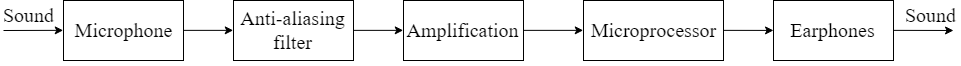
\includegraphics[width=1\textwidth]{highLeveLSystemDiagram.png}
	\caption{Full system block diagram}
	\raggedright
	\label{fig:block}	
\end{figure*}

The microprocessor block consists of all of the signal processing required for the functioning of the hearing aid. The required signal processing is expanded upon in \figref{fig:microBlock}.

\begin{figure*}[t]
	\centering
	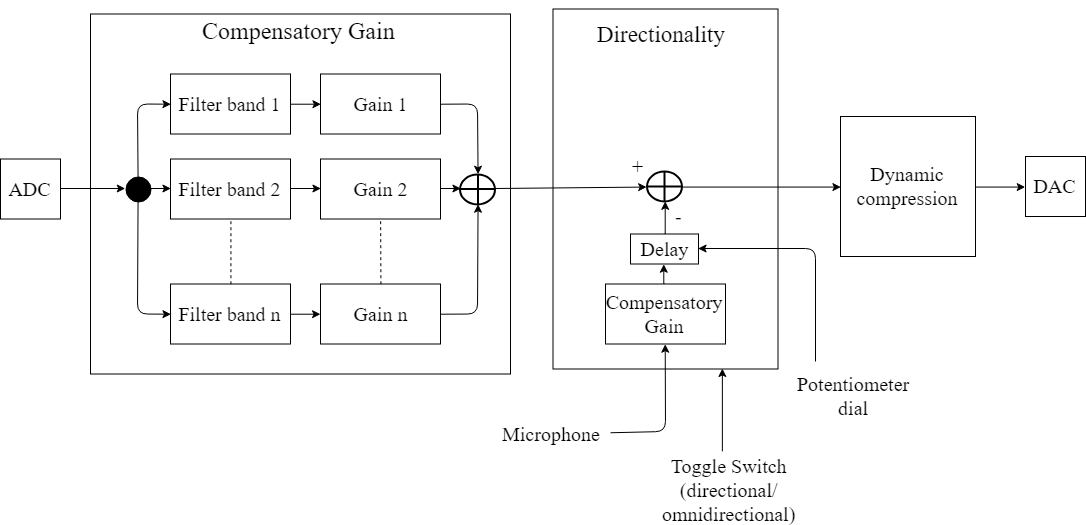
\includegraphics[width=0.8\textwidth]{microBlockDiagrm.png}
	\caption{Block diagram of the software components of the hearing aid}
	\raggedright
	\label{fig:microBlock}	
\end{figure*}

The software components of the system will be programmed using MATLAB and Simulink and thereafter burned onto the Arduino Due microcontroller. By using Simulink, the Arduino can be programmed to function autonomously without needing to be connected to a laptop.

\subsection{Compensatory Amplification} \label{sec:amplification}
In performing the auditory compensatory, amplification will only be applied to the frequency range of speech. As such, 18 filters will be used, each with a bandwidth of 1/3 of an octave. Since phase relationships are crucial in implementing directionality, FIR filters will be used for their linear phase response. In complying with the ANSI standards for filters, third order filters will be used, implying an attenuation of 60dB/decade.

The input signal from each microphone (in directional mode) and from the front microphone (in omni-directional mode) will be passed through the filter bank. This will result in 18 bands of the signal being isolated from one another. Thereafter, a gain matching the audiogram for that frequency range will be applied to each band. In doing so, each signal in the band is multiplied by the gain. Thereafter, each signal is compared to the comfort threshold, and if it exceeds the threshold, its amplitude is reduced until it equals the threshold. Finally, the resultant signals will be added together to produce the compensated signal. 

In order to calculate the required gains for each frequency band, the audiogram requires linear interpolation to increase the resolution as an audiogram only consists of 12 points. In order to ensure that the shape of the audiogram is maintained, a large number of points are required (greater than 1000). The gain for each frequency band will then be selected as the gain on the interpolated audiogram corresponding to the nominal centre frequency of the band.

\subsection{Directionality} \label{sec:directionality}
In order to achieve tunable directionality, a software directional microphone will be used. In the software directional microphone, the signals from two omni-directional microphones are captured and combined in order to create a directional pattern \cite{Distortion_of_interaural_time_cues}. The two microphones will be situated in front and behind the hearing aid device. A desirable directional pattern will be acquired by delaying the signal acquired by the rear microphone and subtracting it from the signal acquired from the front microphone. This configuration is known as a differential microphone array \cite{Distortion_of_interaural_time_cues}.

The directionality feature will be designed such that the user will be able to specify the desired direction of amplification using a potentiometer dial. The analog output voltage of the dial will be read by the ADC of the microcontroller and converted to a time delay. This time delay will be applied to the rear microphone signal and subtracted from the front microphone signal. Thereafter, the direction of maximum gain will be in the same direction that the potentiometer dial is pointing. A block diagram showing this process can be found in \figref{fig:directionalityBlockDiagram}.

\begin{figure}[h]
	\centering
	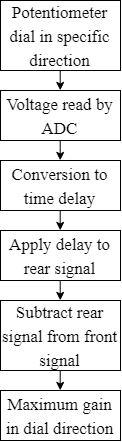
\includegraphics[width=0.3\columnwidth]{directionalityBlockDiagram.png}
	\caption{Block diagram of user tunable directionality feature}
	\raggedright
	\label{fig:directionalityBlockDiagram}	
\end{figure}

In order to create a software directional microphone, certain physical configurations need to be adhered to. One of these considerations is that of the inter-microphone distance \textit{d}. This distance must be equal to half of the wave length of the frequency of interest \cite{Distortion_of_interaural_time_cues}. Since the speech frequency range is of interest, the half wavelength of the centre of the speech range is chosen as the separation distance between the two microphones. Therefore this distance will be 42.875~mm assuming that the speed of sound, \textit{c}, is 343~$m.s^{-1}$.

The directional pattern of a hyper-cardioid is expected to be sufficient to amplify sounds coming from the the direction of interest to the user while attenuating noise from other directions. If it is assumed that the front of the hearing aid device is 0\textdegree, the time delay is required to be equal to $\frac{d}{c}$ to ensure that maximum amplification in the 0\textdegree direction and maximum attenuation in the 180\textdegree direction are experienced \cite{Distortion_of_interaural_time_cues}. The polar pattern plot for this case can be found in Figure~. The direction of the polar pattern maximum will be manipulated by varying the time delay using the potentiometer dial. 

\begin{figure}[h]
	\centering
	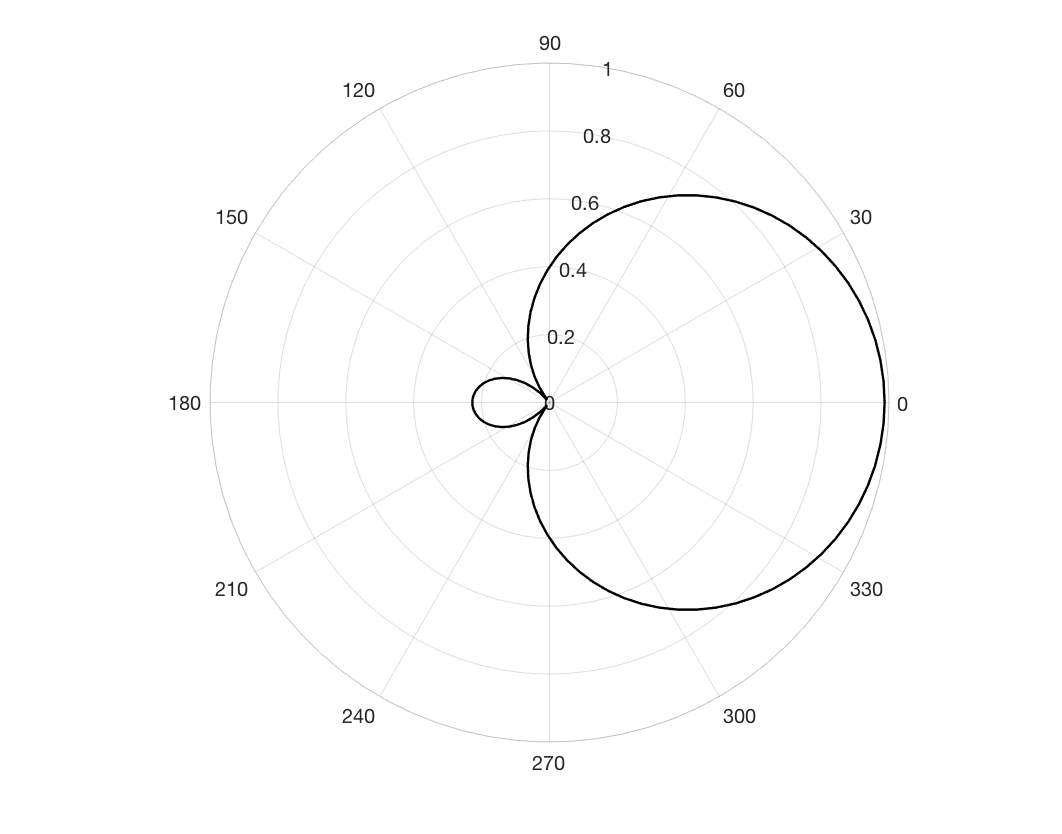
\includegraphics[width=0.9\columnwidth]{polarPlot.png}
	\caption{A hyper-cardiod polar plot}
	\raggedright
	\label{fig:polar}	
\end{figure}

\subsection{Hardware} \label{sec:hardware}
Analog circuitry is required to acquire the sound signal, condition it and convert it to digital. To acquire the signal, two omni-directional microphones are used. The front microphone is the primary microphone which is used alone when the omni-directional mode is selected. The rear microphone is used along with the front microphone when directional mode is selected. The signals from the microphones are amplified and then passed through an eighth order switched capacitor anti-aliasing filter. The filter has a cutoff frequency of 25~kHz, which was selected to ensure that the entire audible range is left unattenuated, while still attenuating the unwanted signal components. Once the signals have been filtered, they are converted to digital by the analog to digital converter (ADC) of an Arduino Due microcontroller. Thereafter, the signals undergo signal processing, as discussed above, before being converted back to analog signals by the Arduino's digital to analog converters. The analog signal corresponding to ear each is then relayed to the appropriate ear using earphones which interact with a headphone jack.

In order to tune the directionality of the hearing aid, a potentiometer, which acts as a dial, will be used. The signal from the potentiometer is also converted to digital by the ADC for signal processing. The hearing aid will include a power button to turn the device on or off, and a toggle switch to switch between directional and omni-directional amplification modes. The entire system will be powered using rechargeable batteries. 

A circuit diagram of the hardware components of the system is given in \figref{fig:circuit}.

	\begin{figure*}[t]
	\centering
	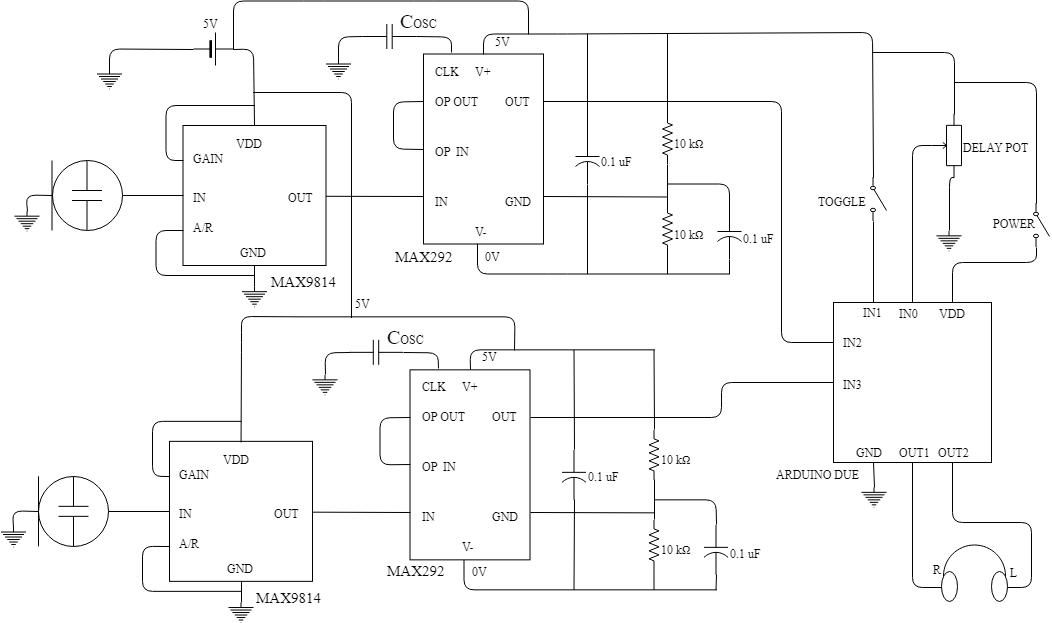
\includegraphics[width=1\textwidth]{fullCircuitDiagram.png}
	\caption{Circuit diagram for the system}
	\raggedright
	\label{fig:circuit}	
\end{figure*}

\subsection{Laboratory Full System Testing} \label{sec:laboratory}
In order to obtain objective results that are free from human bias, the system will be tested in a laboratory using a signal generator to generate pure tones. By generating pure tones of specific frequencies and feeding these tones to the hearing aid, the ability of the device to apply compensatory amplification, and to apply amplification to the correct frequencies, can be quantified. The frequency of the sinusoidal pure tone signals will be set to range from the lower to the upper bounds of the frequency range of human hearing. Additionally, high frequency noise will be added to the signals such that the performance of the device can be evaluated in the presence of noise.

In order to test the directionality of the device, one speaker will be placed in a fixed position. The hearing aid (without the earphones) will be placed in the centre of a rotating platform with the dial facing towards the speaker. A pure tone signal is played from the speaker and the resulting output signal from the hearing aid is saved. The platform is then rotated by 5\textdegree\ and the procedure is repeated. This is done for a 360\textdegree\ range. Once signals have been acquired corresponding to each 5\textdegree\ increment, a polar plot of the signals will be created. In the polar plot, the angle of the signals is taken as the angle of the hearing aid relative the dial (the 0\textdegree\ reference point). This will allow for an analysis of the degree of amplification and attenuation of signals in all directions with the directionality being fixed in one direction.

\subsection{Clinical Full System Testing} \label{sec:clinical}
In order to verify the performance of the hearing aid, clinical tests are required. This will allow for a quantification of the value that the hearing aid provides to the participant.

The method of the clinical testing will now be detailed. First, staff from the school of Electrical and Information Engineering will be asked to participate in the clinical testing. Prior to performing the tests, an audiogram will be collected from each participant using the KUDUwave headset. A hearing aid will then be customised for each participant. Thereafter, a second audiogram will be obtained with the participant wearing the hearing aid. Since the KUDUwave cannot be used on top of earphones, the microphone will be mounted on a model head (made out of polystyrene) and the KUDUwave headset will be placed on top of the fake head. The participant will then wear the earphones which receive the processed signals and a second audiogram will be obtained. The two audiograms will then be compared in order to assess the effectiveness of the compensatory amplification in the device.

\begin{figure}[h]
	\centering
	\begin{subfigure}[t]{0.5\textwidth}
		\centering
		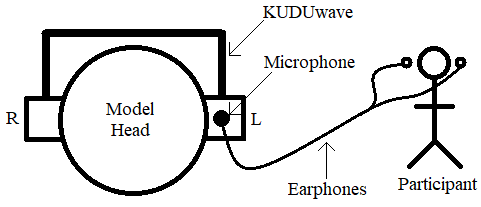
\includegraphics[width=0.8\columnwidth]{gainTestingLeft.png}
		\caption{Testing the left ear}
	\end{subfigure}%
	\\
	\begin{subfigure}[t]{0.5\textwidth}
		\centering
		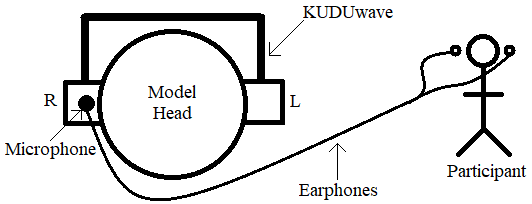
\includegraphics[width=0.8\columnwidth]{gainTestingRight.png}
		\caption{Testing the right ear}
	\end{subfigure}
	\caption{Schematic of the procedure for testing compensatory amplification}
	\label{fig:testing}	
\end{figure}

In order to test the directionality of the device, eight speakers will be set up in a circle, separated by 45\textdegree\ angles. The participant will be asked to sit in a chair which faces 0\textdegree\  while wearing the hearing aid. Pure tone sounds will be played from a single speaker at a time and the participant will be asked to tune the dial controlling the directionality until the sound is at its loudest. The angle of the dial will then be recorded and compared to the angle of the speaker, thus allowing for a quantification of the error present in the directionality. 

\section{PROJECT METHODOLOGIES AND MANAGEMENT}
\subsection{Project Phases}
The project has been divided into 11 development phases, which encapsulate the entire project, from ethics clearance to the presentation. Three of these phases occurred prior to the submission of this document. The phases are detailed in the following sections.

\subsubsection*{Phase 1: Obtain Ethics Clearance} $    $

This phase involved obtaining ethics clearance for the project. This clearance is necessary for clinical testing of the hearing aid, using human input. The procedure for obtaining clearance involves setting out the testing procedure, creating consent forms and creating the questionnaire's for the participants to complete. This phase was completed between the \nth{29} March and the \nth{6} April. Ethics clearance was granted on the \nth{11} May. Both partners were involved in the completion of this phase.

\subsubsection*{Phase 2: Research} $    $

This phase involved performing the research for the project. This included research into compensatory gain, directionality, filtering and the conversion of digital signals to sound signals. This phase occurred from the \nth{25} June to the \nth{1} July. However, it must be noted that research will be an ongoing process throughout the entire duration of the project. Kayla-Jade performed research into gain and filtering and Kelvin investigated directionality and conversions. Thereafter, the research was shared and both partners familiarised themselves with both sets of research.

\subsubsection*{Phase 3: Hardware Design } $    $

In this phase, the circuit diagrams required in the project were designed. The overall system circuit diagram is given in \figref{fig:circuit}. This phase was completed between the \nth{2} July and the \nth{6} July. The two partners performed this phase together.

\subsubsection*{Phase 4: Construction of Hardware } $    $

This phase involves the construction of the circuit that was designed in Phase 3. The circuit will be prototyped on a breadboard before being finalised on a PCB board. The phase will begin on the \nth{9} of July and will end on the \nth{16}. Kelvin will perform the construction of the hardware.

\subsubsection*{Phase 5: Implementation of Compensatory Amplification} $    $

In this phase, the compensatory amplification aspect of the hearing aid will be implemented. This phase has numerous sub-phases:
\begin{itemize}
	\item Sub-phase 1: Interpolation of audiograms and selection of the gains for each filter based on the audiogram
	\item Sub-phase 2: Development of the filter bank
	\item Sub-phase 3: Dynamic compression
	\item Sub-phase 4: Code for ADC and DAC
	\item Sub-phase 5: Optimisation of code from the previous stages to allow for real-time signal processing
\end{itemize}

The first two sub-phases will be implemented by Kayla-Jade. Kelvin will implement sub-phases 3 and 4. The two partners will implement sub-phase 5 together.

The phase will be completed between the \nth{9} of July and the \nth{27} of July.


\subsubsection*{Phase 6: Implementation of the Software Required for Directionality} $    $

In this phase, the software required to implement directionality will be implemented. This software will interface with the dial built into the hardware to tune the direction in which the sound must be amplified. The two partners will implement this phase together. 

This phase will be completed between the \nth{28} of July and the \nth{5} of August.

\subsubsection*{Phase 7: Laboratory testing of the full system} $    $

Following the implementation of the entire system, full system testing is required. 

Both partners will perform the laboratory testing from the \nth{6} until the \nth{10} of August.

\subsubsection*{Phase 8: Clinical testing of the full system} $    $

Phase 7 involves the testing of the audiogram in a clinical setting, using human participants. The procedure to be implemented in this phase is that described in \secref{sec:clinical}

Both partners will perform the clinical testing. The phase will occur between the \nth{13} and the \nth{21} of August.

\subsubsection*{Phase 9: Demonstration} $    $

This phase involves the preparation for open day. This includes creating a poster and a video explaining the project. It also includes preparing the demonstration for open day. Both partners will be involved in all aspects of the phase.

Phase 9 will be completed from the \nth{22} to the \nth{28} of August.

\subsubsection*{Phase 10: Documentation} $    $

This phase involves the writing of the final project report. The report will be worked on throughout the entire project, but in this phase, it will be the sole focus. The partners will each work on their reports individually. 

Phase 10 will be completed from the \nth{29} of August to the \nth{2} of September.

\subsubsection*{Phase 11: Presentation} $    $
Phase 11 is the final phase of the project which involves the preparation of the presentation. This will be done by the partners together. The phase will occur between the \nth{3} and the \nth{12} of September.

\begin{figure*}[h]
	\centering
	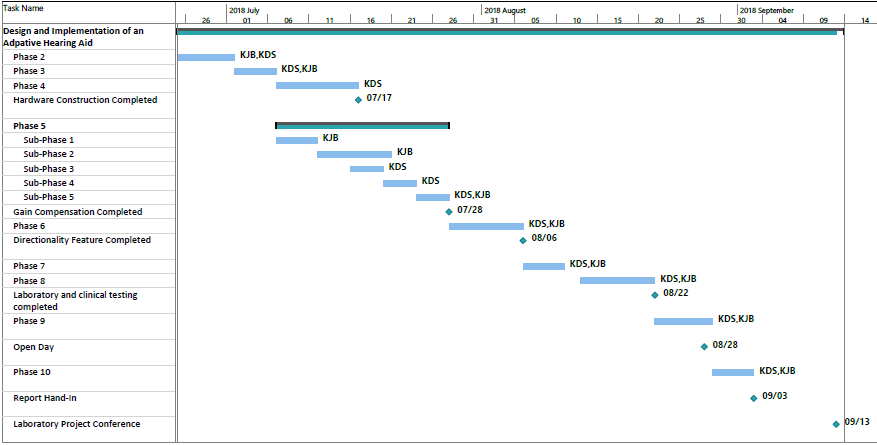
\includegraphics[width=1\textwidth]{GanttChart.png}
	\caption{Gantt chart of the project.}
	\raggedright
	\label{fig:ganttChart}	
\end{figure*}



\section{PROJECT RISK ANALYSIS}

Since the equipment used to obtain an audiogram (the KUDUwave) will need to be obtained from an eMoyo, the group is not in control of its availability. If the equipment is not available, pre-recorded audiograms will be utilized. This will imply that clinical testing will not be possible, since audiograms are required for each participant.

Furthermore, signal generators are required for producing sinusoidal signals for testing. These devices will be obtained from the School of Electrical and Information engineering, as such as, might not be available during the week when testing is scheduled to occur. To mitigate this risk, the required equipment will be booked well in advance to ensure its availability.

The earphones to used with the hearing aid are earphones that are obtained with the purchase of a cell phone. An assumption is being made that these earphones are of a high enough quality to effectively deliver the sound. If this is found to be an incorrect assumption, high quality earphones will need to be purchased, which poses the risk of exceeding the group's budget.

A large risk in the project is that of not having enough time to complete all the phases. In this situation, the phase that would be most severely compromised would be the clinical testing. However, since laboratory testing would have already been performed, the device would have been thoroughly tested. As such, the omission of this phase is not detrimental to the success of the project.

\section{PROJECT COST ANALYSIS}
A breakdown of the components and resources required for the implementation and testing of the hearing aid are given in \tabref{tab:cost}. The table includes the cost of each component and the total cost of the system. The system is estimated to cost R1528, with the cost of components to be purchased being R853.

\begin{table*}[t]
	\centering
	\caption{Cost breakdown for the digital hearing aid}
	\label{tab:cost}
	\begin{tabular}{cccc}
		\cline{2-4}
		\multicolumn{1}{c|}{Purchased Components:}   & \multicolumn{1}{c|}{\textbf{Component}} & \multicolumn{1}{c|}{\textbf{Quantity}} & \multicolumn{1}{c|}{\textbf{Cost (R)}} \\ \cline{2-4} 
		\multicolumn{1}{c|}{} &  \multicolumn{1}{c|}{MAX9814}          & \multicolumn{1}{c|}{2}         & \multicolumn{1}{c|}{240}         \\ \cline{2-4} 
		\multicolumn{1}{c|}{}            & \multicolumn{1}{c|}{Headphone Jack}          & \multicolumn{1}{c|}{1}         & \multicolumn{1}{c|}{17}         \\ \cline{2-4} 
		\multicolumn{1}{c|}{}         &
		\multicolumn{1}{c|}{MAX292}            & \multicolumn{1}{c|}{2}          & \multicolumn{1}{c|}{296}    \\ \cline{2-4} 
		\multicolumn{1}{c|}{}         &
		\multicolumn{1}{c|}{Miscellaneous}            & \multicolumn{1}{c|}{-}           & \multicolumn{1}{c|}{300}    \\ \cline{2-4} 
		& \multicolumn{1}{c|}{}          & \multicolumn{1}{c|}{Subtotal:}         & \multicolumn{1}{c|}{853}         \\ \cline{3-4} 
		&                                &                               &                               \\ \cline{2-4} 
		\multicolumn{1}{c|}{Pre-owned Resources:}   & \multicolumn{1}{c|}{\textbf{Component}} & \multicolumn{1}{c|}{\textbf{Quantity}} & \multicolumn{1}{c|}{\textbf{Cost (R)}} \\ \cline{2-4} 
		\multicolumn{1}{c|}{} & \multicolumn{1}{c|}{Arduino Due}          & \multicolumn{1}{c|}{1}         & \multicolumn{1}{c|}{675}         \\ \cline{2-4} 
		\multicolumn{1}{c|}{}            & \multicolumn{1}{c|}{Earphones}          & \multicolumn{1}{c|}{1}         & \multicolumn{1}{c|}{ - }         \\ \cline{2-4} 
		\multicolumn{1}{c|}{}            & \multicolumn{1}{c|}{Speakers}          & \multicolumn{1}{c|}{8}         & \multicolumn{1}{c|}{ - }         \\ \cline{2-4}
		\multicolumn{1}{c|}{}            & \multicolumn{1}{c|}{Signal Generator}          & \multicolumn{1}{c|}{1}         & \multicolumn{1}{c|}{ - }         \\ \cline{2-4}
		\multicolumn{1}{c|}{}            & \multicolumn{1}{c|}{KUDUwave}          & \multicolumn{1}{c|}{1}         & \multicolumn{1}{c|}{ - }         \\ \cline{2-4}
		& \multicolumn{1}{c|}{}          & \multicolumn{1}{c|}{Subtotal:}         & \multicolumn{1}{c|}{853}         \\ \cline{3-4} \\ \hline
		\multicolumn{1}{c}{\textbf{Total cost:}}             & \multicolumn{1}{l}{}           & \multicolumn{1}{l}{}          & \multicolumn{1}{c}{\textbf{R1528}}  
	\end{tabular}
\end{table*}

\section{CONCLUSION}
The design and project plan for the implementation of an adaptive hearing aid has been presented. The main components of the project are the implementation of compensatory amplification, directionality and the development of the required hardware. The final essential component is the testing of the device, consisting of laboratory and clinical testing. The project will be implemented using MATLAB and Simulink and will make use of an Arduino Due microcontroller. The overall cost of the project is expected to be R1528. The main risks to the project are the lack of availability of the resources needed to test the device.

\bibliographystyle{witseie}
\bibliography{labproject}

\end{document}